% !TEX root = ../../main.tex


\begin{figure}[!htb]
{\footnotesize\texthv{\textbf{(a)}  Misclassification rate}} \\
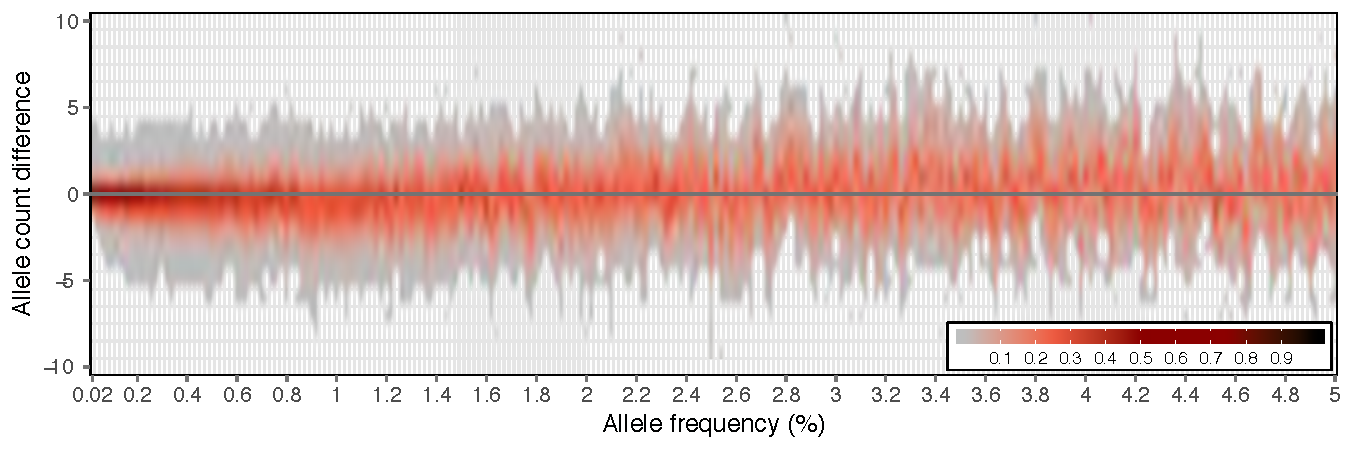
\includegraphics[width=\textwidth]{./img/ch4/fk_error_A_new}
{\footnotesize\texthv{\textbf{(b)}  False positive and false negative rates}} \\
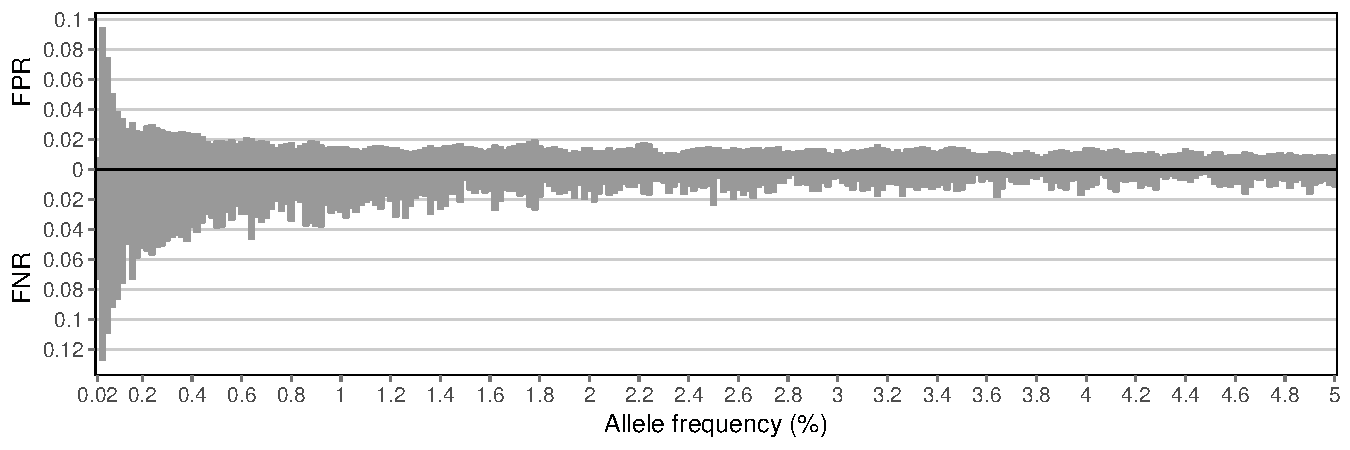
\includegraphics[width=\textwidth]{./img/ch4/fk_error_B}
\Caption{Misclassification of target sites in presence of genotype error}
{Simulated data were modified such that realistic distributions of genotype error were induced.
Panel~\textbf{{(a)}} indicates the rate at which alleles were observed at different frequencies after the inclusion of error.
The proportion of misclassification is indicated by colour intensity.
Panel~\textbf{{(b)}} distinguishes alleles that were falsely observed (false positive) as well as alleles that were missed after the inclusion of error (false negatives).}
{fig:fk_error}
\end{figure}
